%%%%%%%%%%%%%%%%%%%%%%%%%%%%%%
% LATEX-TEMPLATE PROJECTPLAN
%-------------------------------------------------------------------------------
% Voor informatie over het projectplan, zie
% http://practicumav.nl/project/projectplan.html
% Voor readme en meest recente versie van het template, zie
% https://gitlab-fnwi.uva.nl/informatica/LaTeX-template.git
%%%%%%%%%%%%%%%%%%%%%%%%%%%%%%

%-------------------------------------------------------------------------------
%	PACKAGES EN DOCUMENT CONFIGURATIE
%-------------------------------------------------------------------------------

\documentclass{uva-inf-article}
\usepackage[dutch]{babel}
\usepackage{caption}
\usepackage{graphicx}

%-------------------------------------------------------------------------------
%	GEGEVENS VOOR IN DE TITEL
%-------------------------------------------------------------------------------

% Vul de naam van de opdracht in.
\assignment{Projectplan}
% Vul het soort opdracht in.
\assignmenttype{Projectplan}
% Vul de titel van de eindopdracht in.
\title{MyEcology}

% Vul de volledige namen van alle auteurs in.
\authors{Valentyn Gnativ; Elias Dekker; Milou Hermes; Kim Roks; Joseph Krol}
% Vul de corresponderende UvAnetID's in.
\uvanetids{14609037; 14638487; 14375915; 14617811; 14328968}

% Vul altijd de naam in van diegene die het nakijkt, tutor of docent.
\tutor{Robin Slot}
% Vul eventueel ook de naam van de docent of vakcoordinator toe.
\docent{Dr Yuri Demchenko}
% Vul hier de naam van de groep  in.
\group{Inf 16}
% Vul de naam van de cursus in.
\course{Webtechnologie}
% Te vinden op onder andere Datanose.
\courseid{5082WEBT6Y}

% Dit is de datum die op het document komt te staan. Standaard is dat vandaag.
\date{\today}

%-------------------------------------------------------------------------------
%	VOORPAGINA
%-------------------------------------------------------------------------------

\begin{document}
\maketitle

%-------------------------------------------------------------------------------
%	INHOUDSOPGAVE
%-------------------------------------------------------------------------------

\tableofcontents

%-------------------------------------------------------------------------------
%	ACHTERGROND
%-------------------------------------------------------------------------------

\section{Achtergrond}
% is nog te kort
% inspiratie
% Lecture 1 dia's 33 en 34
Onze vraag is of we aan de hand van onze website de ecologische voetafdruk van individuen in kaart kunnen brengen, en of het mogelijk is om zo mensen op de hoogte te stellen van hun uitstoot en welke stappen ze kunnen nemen om deze te verminderen.
Dit is geïnspireerd door o.a. de klimaatdoelen die vastgesteld waren in de COP26 klimmaattop. Hierin werd voorgenomen om de netto CO2-uitstoot op een globaal niveau naar nul te brengen.
De ecologische voetafdruk geeft aan wat de uitstoot van broeikasgassen van iets is. In dit geval is dit de uitstoot van de individuele gebruiker van de website. De hoeveelheid van deze uitstoot wordt bepaald door wat een persoon doet en consumeert op een dag.

%-------------------------------------------------------------------------------
%	DOELEN
%-------------------------------------------------------------------------------

\section{Projectdoelstelling}


\subsection{Doelstelling}
De doelstelling voor dit project is het maken van een website waarmee bezoekers op een eenvoudige manier hun eigen ecologische impact kunnen vergelijken. Bezoekers kunnen een account aanmaken, een tijdsinterval kiezen en antwoord geven op een aantal vragen. Welke vragen hiervoor worden gekozen, zullen we nog verder uitwerken met behulp van betrouwbare bronnen.
\subsubsection{privacy}
Het is belangrijk dat er op een goede en veilige manier met de informatie die gebruikers ons geven wordt omgegaan. Deze gegevens mogen alleen gebruikt worden om de ervaring van onze gebruikers te verbeteren. De informatie mag niet zonder duidelijke reden gedeeld worden. Wij respecteren ieders recht op privacy.


\subsection{Visie}
Het idee is om mensen een overzicht te geven over hun ecologische voetafdruk. Met deze informatie is het overzichtelijk hoeveel iedere persoon uitstoot en wat er aan gedaan kan worden om die uitstoot te verminderen. Daarom is onze visie het verbeteren van het klimaat door duurzamer te leven.

%-------------------------------------------------------------------------------
%	RESULTAAT
%-------------------------------------------------------------------------------

\section{Projectresultaat}
Als eindresultaat verwachten wij een volledig werkende website, die gelijk online zou kunnen worden geplaatst. Onze website gaan we ook zeker online plaatsen, aangezien wij al een domeinnaam gekocht hebben. Omdat wij van competitie houden, willen we ook proberen om voor de beste website te gaan. Als deze dingen ons zouden lukken, dan verwachten wij ook minimaal een 8 als eindcijfer. 

%-------------------------------------------------------------------------------
%	ORGANISATIE
%-------------------------------------------------------------------------------

\section{Projectorganisatie}
\subsection{Rollen} 
De instructie was gegeven bij dit project om rollen te verdelen op een specifieke manier. Deze rollen zijn zo vormgegeven: 
\begin{itemize}
    \item Github expert: Kim. De taak van de Github expert is om alle samenwerking met Github goed te laten verlopen en als er problemen zijn deze zo snel mogelijk op te lossen.
    \item Facilitator: Elias en Valentyn. De taak van de facilitator is om te zorgen dat alle taken volgens de planning verlopen en ruimtes te reserveren.
    \item Serverbeheerder: Joseph. Alle zaken betreffende de server in goede banen leiden.
    \item Voorzitter: Joseph. Leidt vergaderingen en verdeelt taken.
    \item Notulist: Milou. Verwerkt progressie en noteert deze ontwikkelingen. 
\end{itemize}

\subsection{Communicatie}
Wij hebben afgesproken om voor communicatie tijdens dit project, de volgende hulpmiddelen te gebruiken:
\begin{itemize}
    \item Trello
    \item Discord
    \item MS Teams
    \item Telegram
    \item Overleaf
\end{itemize}

\subsection{Andere programma's en informatiebronnen}
Wij zijn van plan om voor het functioneren van de website gebruik te maken van een API en een database. De database is te vinden op  \url{https://world.openfoodfacts.org}, hierin staat over een enorme hoeveelheid voedingsproducten informatie over hoeveel uitstoot het produceren en vervoeren van het product heeft voortgebracht.
De API is te vinden op \url{https://data.footprintnetwork.org/\#/api}.
Door deze API zijn wij in staat om per locatie, de gemiddelde voetafdruk op te vragen, zodat gebruikers hun eigen uitstoot kunnen vergelijken met de uitstoot van anderen.

\subsection{Verantwoording van geleverd werk}
\begin{figure} [h]
    \centering
    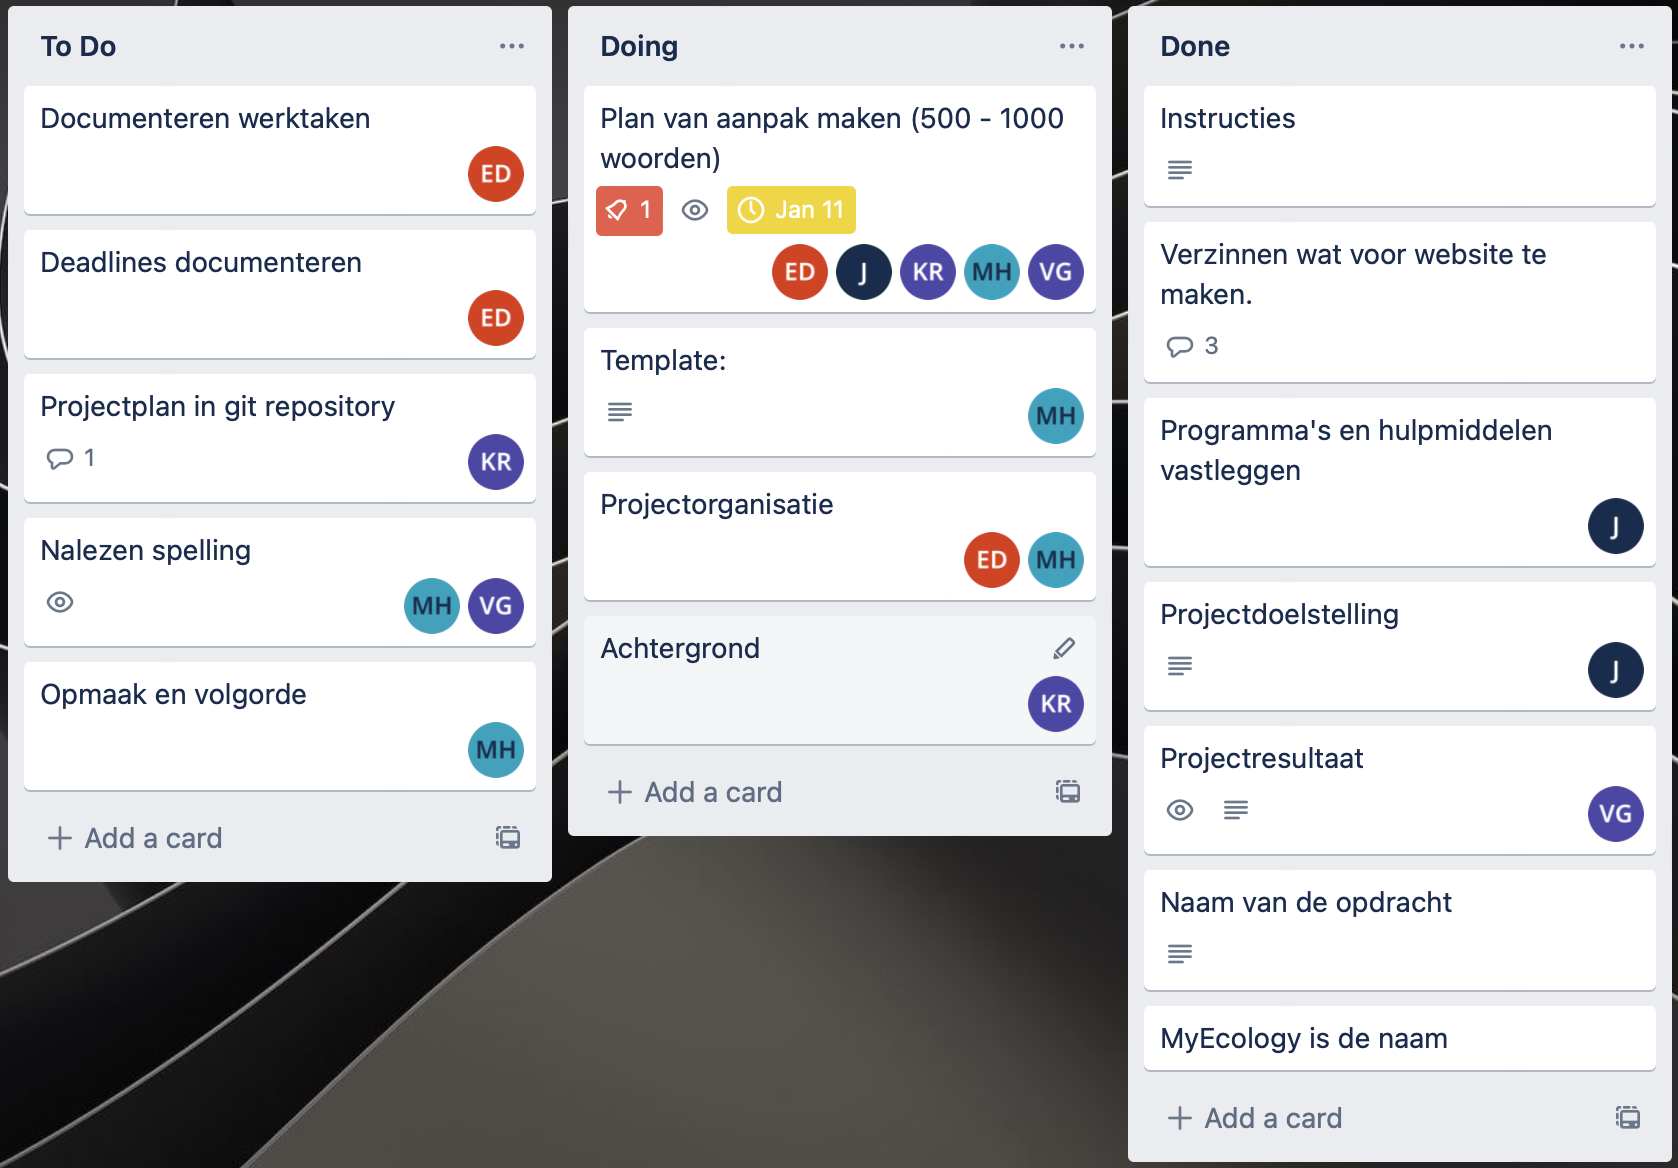
\includegraphics[scale=0.4]{trello.jpg}
    \caption{Screenshot van Trello}
    \label{fig:my_label}
\end{figure}
\break{}
\subsection{Werkafspaken}
\textit{Concept van deadlines:}

\begin{table} [h]
\centering
\captionsetup{labelformat=empty}
\begin{tabular} {lll} 
Dag        &                                                                                                             &                                                                                                                                                                                 \\
15 januari & \begin{tabular}[c]{@{}l@{}}HTML/CSS, \\Javascript, pen en papier,\\gedeeld online document\end{tabular}     & \begin{tabular}[c]{@{}l@{}}Prototype structuur en design,\\beschrijving van data die gebruikt wordt en uitgewisseld.\end{tabular}                                               \\
22 januari & \begin{tabular}[c]{@{}l@{}}MySQL, \\phpMyAdmin en PHP\end{tabular}                                          & \begin{tabular}[c]{@{}l@{}}Website design afmaken, data toevoegen\\en usage experience. Backend database is werkend en\\ondersteund de web applicatie.\end{tabular}             \\
29 januari & \begin{tabular}[c]{@{}l@{}}PHP, Javascript, \\AJAX, externe data met\\WebAPI en web \\scraping\end{tabular} & \begin{tabular}[c]{@{}l@{}}User facing interface en services, \\website debugging en fixing. \\WebAPI en/of web scraping \\geïmplenteerd en getest.\end{tabular}                \\
5 februari & \begin{tabular}[c]{@{}l@{}}Final testing en \\writing report\end{tabular}                                   & \begin{tabular}[c]{@{}l@{}}Checken en toepassen security \\considerations. \\Web application is klaar and volledig\\getest, het verslag is klaar, \\demonstratie.\end{tabular}  \\
           &                                                                                                             &                                                                                                                                                                                 \\
           &                                                                                                             &                                                                                                                                                                                
\end{tabular}
\end{table}

%-------------------------------------------------------------------------------
%	PLANNING
%-------------------------------------------------------------------------------

%Zet de planning indien gewenst in een apart document
%\input{planning}

%-------------------------------------------------------------------------------
%	BIJLAGEN EN EINDE
%-------------------------------------------------------------------------------

%\section{Bijlage A}
%\section{Bijlage B}
%\section{Bijlage C}

\end{document}